\section{Marketing and Sales}
Market adoption and sales are the true measures of success. Clearly convey your strategy and tactics to penetrate the market and drive sales. Potential investors want to understand your customer awareness and buying stimulus programs from the customer�s and salesperson�s perspective. If you are not currently selling your product, explain your product launch plans. Convince the audience that you have an effective go-to-market strategy that will not break the bank.

Include the following key points:
checkmark - What is your go-to-market strategy?
- How will you drive market demand for your product?
- What is your branding strategy?
- What is your pricing strategy?
Addressed in Model - What is your marketing communication plan?
checkmark - How will you recruit and build your sales force?
- What is your distribution plan?
Addressed in Model- Who will be your key partners?
checkmark - What is your customer retention strategy?
checkmark- Who are your largest customers?

Refer to the information you have documented in Market Strategy Development Workbook 2: Critical Value Factors and Market Strategy Development Workbook 3: Strategic Marketing Approach.

Describe your go-to-market strategy in the corresponding section of the Business Planning and Executive Summary workbook template. Use the information from the Market Strategy Development workbook guides that is indicated in the bullet list above.



\subsection{The Competition}
To properly evaluate the competition and find our foothold in the market, Table \ref{competition} shows our competition profile.

\begin{table}[ht]
\caption{Defining the Competition} % title of Table
\centering % used for centering table
\begin{tabular}{| p{2in} | p{1in} | p{2in} |} % centered columns (4 columns)
\hline
Competitor & Type of Competition & Strengths \\
\hline % inserts single horizontal line
Previously established approval software contracts. & Economic & Strength: Our product will be easier to justify using in their current budgets.\\ \hline % inserting body of the table space
Document revision control schemes (ie: Google Docs) & Direct & Strength: Our product will focus specifically on the professional challenges associated with establishing a secure approval process. \\
\hline %inserts single line
\end{tabular}
\label{competition} % is used to refer this table in the text
\end{table}

\subsection{How we Differ from the Competition}
We focus on differentiating ourselves from our competitors by providing a product that helps develop a productive and frustration-free work environment. Seeking approval for your work by a higher-up should not be a cumbersome process. Acknowledgements allows users to quickly draft an approval request and send it off in minutes from anywhere. 

Every aspect of our software will focus on helping the customer have a hassle-free experience. The interface will be uncluttered and easy to use. Mobile and desktop web applications will allow for your Acknowledgements account to be easily accessible. Finally, our eager team will be available to help create custom functionality to serve the ever-changing needs of our clients.

Our value curve shows visually how we differentiate ourselves from our competition.

\begin{figure}[ht!]
\centering
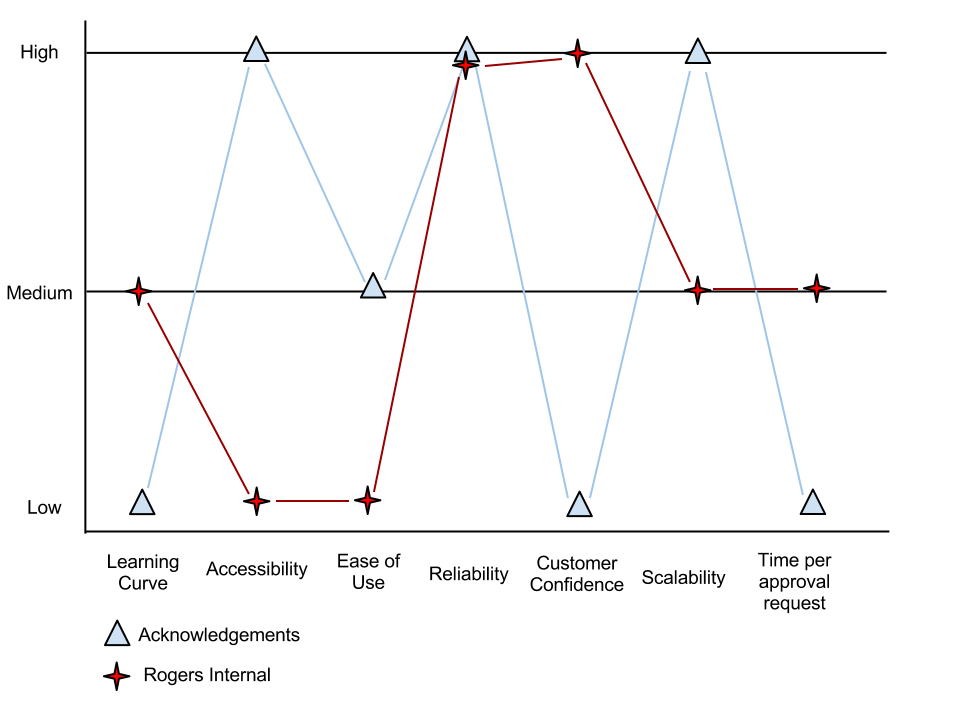
\includegraphics[width=150mm]{images/MSCI454-ValueCurve.png}
\caption{Value Curve}
\label{valuecurve}
\end{figure}

\subsection{Go-to-Market Strategy}

Our go-to-market strategy involves obtaining our first clients by August of 2013. Our entire plan from the early stages of development to the revenue-earning phase is detailed in the following figure.

\begin{figure}[ht!]
\centering
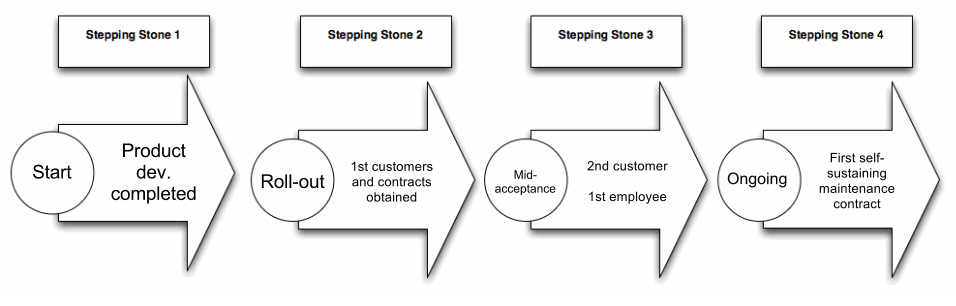
\includegraphics[width=150mm]{images/MSCI454-SteppingStones.png}
\caption{Growth Cycle}
\label{growthCycle}
\end{figure}

We are planning to enter the product development stage by early May 2013. With our experienced team, we will have the product ready for release by mid August 2013.

We will roll-out our product to our first customer by the end of August 2013. Our next set of customers will be obtained by end-of-year 2013.

Once the second customer base is established, we will enter the ongoing phase of our company's growth. Self-sustaining maintenance contracts will be the main source of revenue for the company, and no more funding will be required.

\subsection{Hiring Cycle}

Once {\bf Acknowledgements} has achieved its {\bf Mid-Acceptance} milestone presented in figure \ref{growthCycle} we will hire our first employee. As our second customer base is acquired, the extra work will require the additional employee to help maintain the maintenance contracts.

As {\bf Acknowledgements} grows to its {\bf Ongoing} milestone, it will be time to hire new sales staff. Maintenance contracts will makeup the majority of our work base, and new clients need to be acquired. At this point within our first year, a single sales staff will represent {\bf Acknowledgements} on the market. It will be expected that this staff bring in more clients. 

\subsection{Customer Retention}
Customer retention lends itself well to our market. From our research, companies tend to invest in a particular approval software solution, and then stick with it. This is exemplified by the problem we are trying to address: Companies have blindly stuck with their unacceptable approval software for years because the hassle of changing was undesirable. 

We will capitalize on this mindset by making the migration as easy as possible for our clients. Then, once they are established with our product, the same mindset will be used to justify staying with our product, with the additional advantage of our product meeting all our our clients' needs in a superior way to their previous solutions.

\subsection{Target Customers}
Our target customers are the major Canadian construction firms. The approval process is entrenched in their company's work flow and it is often the case that the software they use for this task is many years outdated. 

Our largest target customers include many of the members of the Canadian Construction Association including:

\begin{enumerate}
  \item AECON Buildings
  \item Hamilton-Halton Construction Association
  \item Infrastructure Ontario
  \item PCL Constructors Inc.
  \item Pennecon Ltd.
\end{enumerate}


